\chapter{Iterazione 1: Implementazione dell'Accounting Service}
\label{chap:iterazione1}

\section{Introduzione e Obiettivi dell'Iterazione}

L'Iterazione 1 del progetto \textit{JarFin} ha rappresentato la fase fondativa dello sviluppo, dedicata alla progettazione e alla realizzazione del microservizio \textbf{Accounting Service}. Questo componente costituisce il nucleo operativo dell'intera architettura, essendo responsabile della gestione autoritativa delle transazioni finanziarie (registrazione, consultazione, modifica e cancellazione).

L'obiettivo primario di questa fase non si è limitato alla semplice implementazione delle funzionalità CRUD (\textit{Create, Read, Update, Delete}), ma ha riguardato la costruzione di un'infrastruttura software solida, basata sui principi della \textit{Clean Architecture} e pronta per supportare la scalabilità futura.
Le sfide principali affrontate hanno riguardato:

\begin{itemize}
    \item \textbf{Infrastruttura}: Configurazione di un ambiente di sviluppo containerizzato e riproducibile tramite Docker.
    \item \textbf{Persistenza}: Gestione rigorosa dei dati su un RDBMS relazionale (PostgreSQL).
    \item \textbf{Architettura}: Definizione di pattern per la validazione, la gestione centralizzata degli errori e il disaccoppiamento dei dati (DTO/Mapper).
    \item \textbf{Qualità}: Garanzia della robustezza del codice tramite una strategia di testing ibrida (Unitari e di Integrazione).
\end{itemize}

\section{Stack Tecnologico e Configurazione}

Il microservizio è stato sviluppato adottando uno stack tecnologico moderno, scelto per garantire robustezza e facilità di manutenzione:

\begin{itemize}
    \item \textbf{Java 21}: Utilizzato come linguaggio di programmazione, sfruttando le ultime funzionalità LTS (\textit{Long Term Support}) per massimizzare performance e sicurezza.
    \item \textbf{Spring Boot 3.2.0}: Framework di riferimento per lo sviluppo di microservizi in ambiente Java. Ha permesso di abbattere i tempi di configurazione (\textit{Convention over Configuration}) fornendo un server web integrato (Tomcat) e la gestione automatica delle dipendenze.
    \item \textbf{Spring Data JPA / Hibernate}: Per la gestione della persistenza tramite ORM (\textit{Object-Relational Mapping}), astraendo la complessità delle query SQL dirette.
    \item \textbf{PostgreSQL 16}: Scelto come RDBMS per la sua affidabilità, il supporto alle transazioni ACID e la capacità di gestire carichi di lavoro complessi.
    \item \textbf{Docker \& Docker Compose}: Per l'orchestrazione dell'ambiente di sviluppo e la containerizzazione del database.
    \item \textbf{Lombok}: Libreria utilizzata per ridurre il codice "boilerplate" (getter, setter, costruttori), migliorando la leggibilità delle classi.
    \item \textbf{Maven}: Per la gestione del ciclo di vita del software e delle dipendenze, come definito nel file \texttt{pom.xml}.
\end{itemize}

\section{Orchestrazione (Docker Compose)}

Una delle prime decisioni architetturali è stata quella di disaccoppiare l'applicazione dall'installazione locale del database. Per garantire che l'ambiente di sviluppo fosse deterministico e identico per ogni sviluppatore, si è optato per la virtualizzazione tramite \textbf{Docker}.

\newpage

Il file \texttt{docker-compose.yml} definisce il servizio di database e le sue configurazioni:

\bigskip

\begin{lstlisting}[language=yaml, label={lst:dockercompose}]
services:
  db:
    image: postgres:15
    container_name: jarfin_db
    environment:
      POSTGRES_USER: ${DB_USER:-postgres}
      POSTGRES_PASSWORD: ${DB_PASSWORD:-password_segreta}
      POSTGRES_DB: jarfin_db
    ports:
      - "5432:5432"
    volumes:
      - postgres_data:/var/lib/postgresql/data

volumes:
  postgres_data:
\end{lstlisting}

\subsection{Analisi delle Scelte Implementative}
\begin{itemize}
    \item \textbf{Persistenza dei Dati}: L'uso di un volume nominato (\texttt{postgres\_data}) garantisce la persistenza dei dati anche in caso di arresto o rimozione dei container, evitando la perdita di informazioni tra le sessioni di sviluppo.
    \item \textbf{Sicurezza delle Credenziali}: Le credenziali di accesso non sono rigidamente fissate nel codice. La configurazione supporta l'iniezione tramite variabili d'ambiente (\texttt{\$\{DB\_PASSWORD\}}), con valori di default visibili solo per facilitare la revisione accademica. Questo approccio predispone il sistema per pipeline CI/CD sicure.
    \item \textbf{Networking}: Il database è esposto sulla porta 5432, permettendo connessioni sia dall'applicazione Spring Boot che da tool di amministrazione esterni (es. DBeaver/pgAdmin).
\end{itemize}

L'applicazione Spring Boot si connette al container in questione tramite il file \texttt{application.properties}, configurato per aggiornare automaticamente lo schema del database all'avvio (\texttt{spring.jpa.hibernate.ddl-auto=update}), accelerando notevolmente la fase di prototipazione.

\section{Architettura Software e Design Patterns}

Il microservizio implementa un'architettura a strati rigorosa (\textit{Layered Architecture}) per garantire la separazione delle responsabilità (\textit{Separation of Concerns}).
Il flusso dei dati attraversa i seguenti layer, in ordine:

\begin{itemize}
  \item \textbf{Controller (API)}: espone gli endpoint REST e gestisce le richieste HTTP;
  \item \textbf{Mapper / DTO}: converte i dati tra il modello di dominio e il contratto API;
  \item \textbf{Service (Business Logic)}: incapsula la logica applicativa;
  \item \textbf{Repository (Data Access)}: gestisce l’accesso e la persistenza dei dati.
\end{itemize}

\subsection{Modellazione del Dominio: La scelta di BigDecimal}
L'entità \texttt{Transaction} rappresenta il concetto centrale del dominio. Durante la modellazione, è stata posta particolare attenzione al tipo di dato per l'attributo \texttt{amount} (importo).

L'uso di tipi primitivi a virgola mobile come \texttt{double} o \texttt{float} è stato scartato a causa dell'imprecisione intrinseca nella rappresentazione binaria dei decimali (standard IEEE 754), che può portare a errori di arrotondamento inaccettabili in ambito finanziario.
È stato quindi adottato \texttt{java.math.BigDecimal}, che garantisce una precisione arbitraria e operazioni aritmetiche esatte.

\bigskip

\begin{lstlisting}[language=Java, label={lst:transactionentity}]
@Entity
@Table(name = "transactions")
@Getter @Setter @NoArgsConstructor
public class Transaction {
    @Id
    @GeneratedValue(strategy = GenerationType.IDENTITY)
    private Long id;

    @Column(nullable = false, precision = 19, scale = 4)
    private BigDecimal amount; // Precisione finanziaria garantita

    @Column(nullable = false)
    private LocalDate date;

    @Enumerated(EnumType.STRING)
    @Column(nullable = false)
    private TransactionType type; // INCOME o EXPENSE
    
    // ... altri campi (description, category)
}
\end{lstlisting}

Inoltre, per evitare problemi noti con i proxy di Hibernate, i metodi \texttt{equals()} e \texttt{hashCode()} sono stati implementati manualmente basandosi strettamente sull'identificatore univoco (\texttt{id}) dell'entità.

\subsection{Pattern DTO e Mapper}
Per disaccoppiare il modello di persistenza (Entity) dal contratto esposto all'esterno (API), è stato implementato il pattern DTO (Data Transfer Object).

\begin{itemize}
    \item \textbf{\texttt{TransactionRequest}}: Utilizzato per l'inserimento dati. Include annotazioni di Jakarta Validation (\texttt{@NotNull}, \texttt{@DecimalMin}, \texttt{@NotBlank}) per garantire che i dati in ingresso siano validi prima ancora di raggiungere la logica di business.
    \item \textbf{\texttt{TransactionResponse}}: Utilizzato per la risposta. Filtra eventuali dati tecnici non necessari al client.
\end{itemize}

La conversione tra Entity e DTO è centralizzata nella classe \texttt{TransactionMapper}, mantenendo il Controller e il Service puliti da logiche di trasformazione dei dati.

\section{Logica di Business e Gestione Errori}

\subsection{Service Layer}
La classe \texttt{TransactionService} incapsula la logica core. Un aspetto rilevante è l'uso dell'annotazione \texttt{@Transactional} sui metodi di modifica, che garantisce l'atomicità delle operazioni sul database: o l'operazione ha successo completamente, o viene eseguito un rollback.
Inoltre, è stato introdotto un sistema di logging (\texttt{@Slf4j}) per tracciare le operazioni critiche, fondamentale per il debugging in un ambiente distribuito.

\subsection{Gestione Centralizzata delle Eccezioni}
Invece di disseminare blocchi \texttt{try-catch} nel codice, è stato implementato un Global Exception Handler utilizzando \texttt{@RestControllerAdvice}.
Questo componente intercetta le eccezioni a livello globale e le trasforma in risposte JSON strutturate con i corretti codici di errore HTTP.

\bigskip

\begin{lstlisting}[language=Java, label={lst:globalhandler}]
@RestControllerAdvice
public class GlobalExceptionHandler {

    // Gestione 404 Not Found
    @ExceptionHandler(EntityNotFoundException.class)
    public ResponseEntity<String> handleNotFound(EntityNotFoundException ex) {
        return ResponseEntity.status(HttpStatus.NOT_FOUND).body(ex.getMessage());
    }

    // Gestione 400 Bad Request (Errori di Validazione)
    @ExceptionHandler(MethodArgumentNotValidException.class)
    public ResponseEntity<Map<String, String>> handleValidationErrors(
            MethodArgumentNotValidException ex) {
        Map<String, String> errors = new HashMap<>();
        ex.getBindingResult().getFieldErrors().forEach(error -> 
            errors.put(error.getField(), error.getDefaultMessage()));
        return ResponseEntity.badRequest().body(errors);
    }
}
\end{lstlisting}

Questo approccio migliora drasticamente l'usabilità dell'API: se un client invia un importo negativo, riceverà un errore 400 chiaro e dettagliato invece di un generico errore 500.

\section{Esposizione API: TransactionController}

Il \texttt{TransactionController} espone le funzionalità tramite endpoint RESTful standard. È stata posta particolare cura nel rispetto della semantica HTTP.
Il metodo \texttt{create}, in particolare, implementa il livello 2 del modello di maturità di Richardson (HTTP Verbs), restituendo l'header \texttt{Location} con l'URI della risorsa appena creata.

\bigskip

\begin{lstlisting}[language=Java, label={lst:createcontroller}]
@PostMapping
public ResponseEntity<TransactionResponse> create(@Valid @RequestBody TransactionRequest request) {
    Transaction entity = mapper.toEntity(request);
    Transaction saved = service.saveTransaction(entity);
    
    // Costruzione dinamica dell'URI della risorsa
    URI location = ServletUriComponentsBuilder.fromCurrentRequest()
            .path("/{id}")
            .buildAndExpand(saved.getId())
            .toUri();

    return ResponseEntity.created(location)
                         .body(mapper.toResponse(saved));
}
\end{lstlisting}

\section{Qualità del Codice e Strategia di Testing}

La validazione dell'Iterazione 1 non si è limitata alla sola verifica funzionale, ma ha seguito un percorso strutturato partendo dall'analisi statica del codice, passando per i test unitari con monitoraggio della copertura, fino ai test di integrazione manuali.

\subsection{Analisi Statica e Refactoring (SonarLint)}

Prima di procedere con il testing dinamico, è stata eseguita un'analisi statica del codice utilizzando \textbf{SonarLint}. Questa fase ha permesso di rilevare violazioni delle convenzioni REST e disuniformità nella gestione delle eccezioni.

\newpage

In particolare:
\begin{itemize}
    \item \textbf{Problema rilevato:} Il \texttt{TransactionController} restituiva status code generici e mancava l'header \texttt{Location} nelle risposte POST, violando le best practices RESTful.
    \item \textbf{Intervento correttivo:} È stato introdotto \texttt{UriComponentsBuilder} ed eseguito un refactoring dei metodi per restituire oggetti \texttt{ResponseEntity} tipizzati correttamente, migliorando la semantica delle API.
\end{itemize}

\begin{figure}[H]
    \centering
    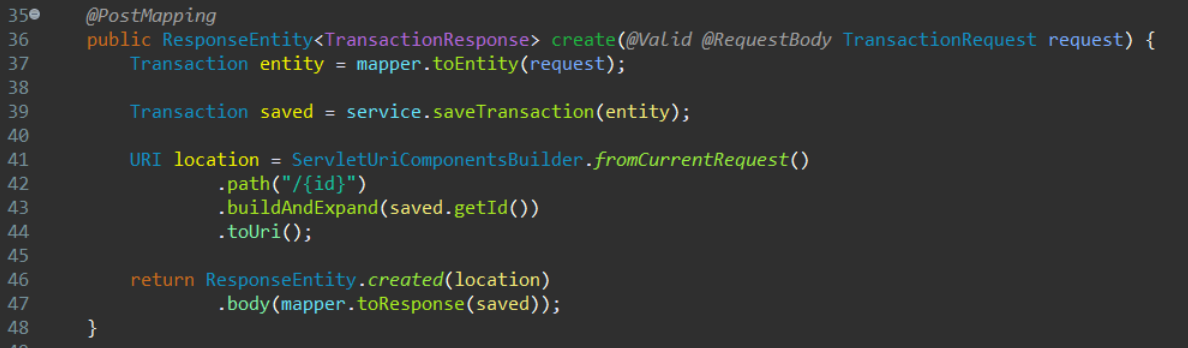
\includegraphics[width=0.9\textwidth]{../Iterazione_1/images/UriComponentsBuilder.png}
    \caption{Refactoring del Controller per conformità REST}
    \label{fig:sonar_refactoring}
\end{figure}

Inoltre, sono state applicate correzioni minori suggerite dal linter, come la rimozione del modificatore \texttt{public} nei metodi di test (Figura \ref{fig:sonar_public}), rendendo il codice più pulito e conforme alle convenzioni di JUnit 5.

\begin{figure}[H]
    \centering
    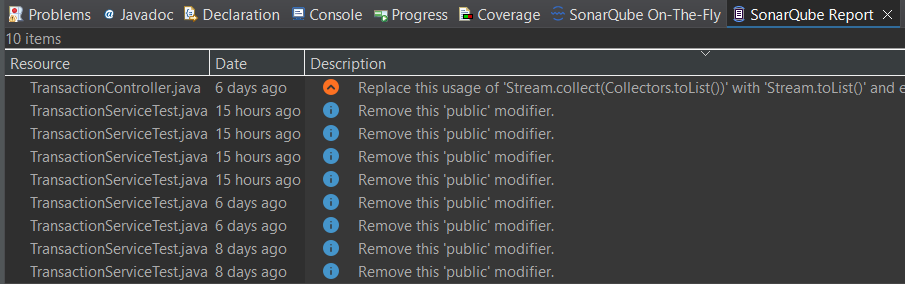
\includegraphics[width=0.9\textwidth]{../Iterazione_1/images/public_modifier.png}
    \caption{Esempio di code smell rilevato da SonarLint}
    \label{fig:sonar_public}
\end{figure}

\subsection{\mbox{Unit Testing e Copertura (JUnit 5, Mockito \& EclEmma)}}

Per la verifica della logica di business, sono stati sviluppati test unitari isolati per il Service e il Controller.
L'uso di \textbf{Mockito} ha permesso di simulare il comportamento del database (pattern \textit{mocking}), verificando la corretta generazione delle risposte HTTP e l'elaborazione dei dati senza dipendenze esterne.

\subsubsection*{Strategia di Copertura}
Non è stato perseguito l’obiettivo formale del 100\% di copertura, ma si è adottato un approccio \textbf{mirato} (soglia minima 85\%), concentrandosi sui metodi critici che:
\begin{itemize}
    \item contengono logica di business non banale o calcoli finanziari;
    \item garantiscono l'integrità dei dati (es. validazione importi negativi);
    \item gestiscono la persistenza e le transazioni verso il database.
\end{itemize}

La Figura \ref{fig:junit} mostra l'esecuzione con successo della suite di test nell'ambiente di sviluppo.

\begin{figure}[H]
    \centering
    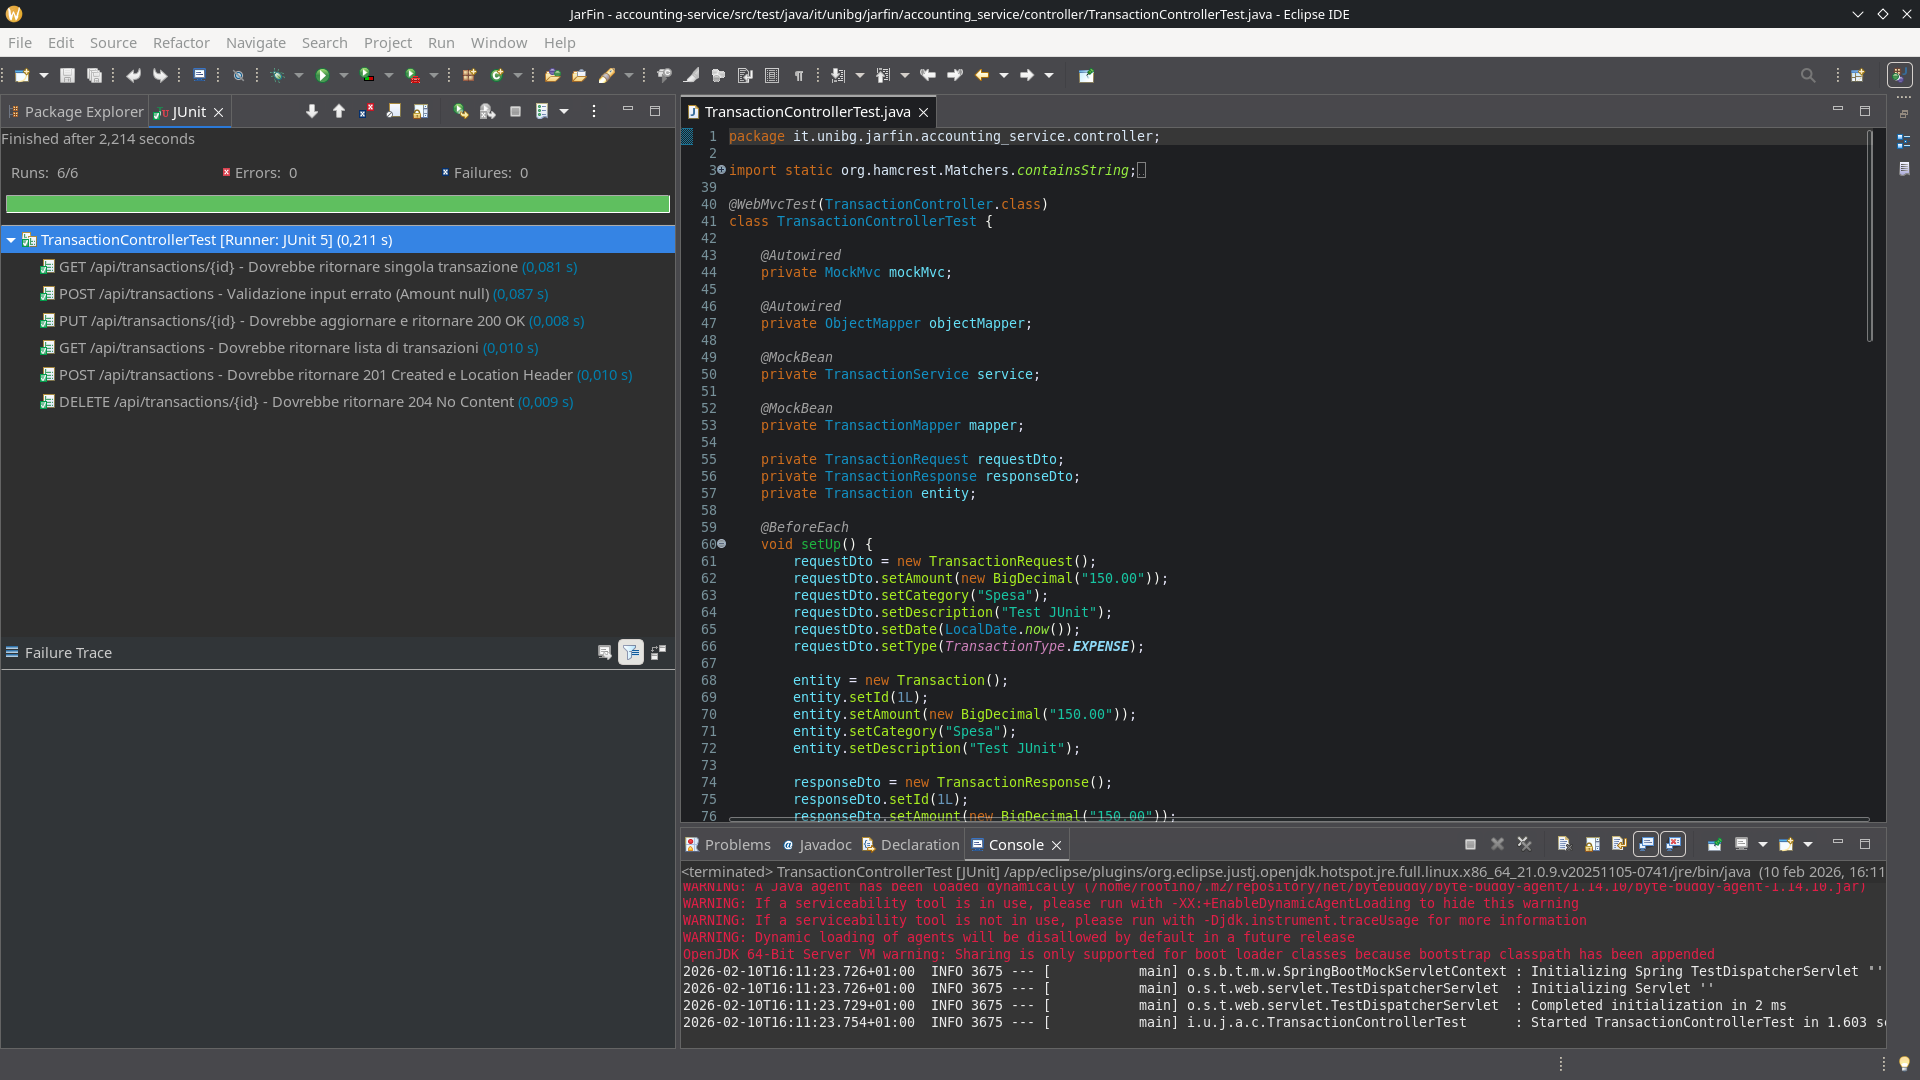
\includegraphics[width=0.9\textwidth]{../Iterazione_1/images/TransactionControllerTest.png}
    \caption{Suite di test unitari completata con successo su TransactionController}
    \label{fig:junit}
\end{figure}

\subsubsection{Metriche Raggiunte}
L'analisi con \textbf{EclEmma} ha confermato l'efficacia della strategia, raggiungendo livelli di copertura eccellenti per il modulo di contabilità:

\begin{itemize}
    \item \textbf{Service Layer Coverage:} 100\%
    \item \textbf{Controller Layer Coverage:} 100\%
    \item \textbf{Accounting Service Package Coverage:} 96\%
\end{itemize}

\begin{figure}[H]
    \centering
    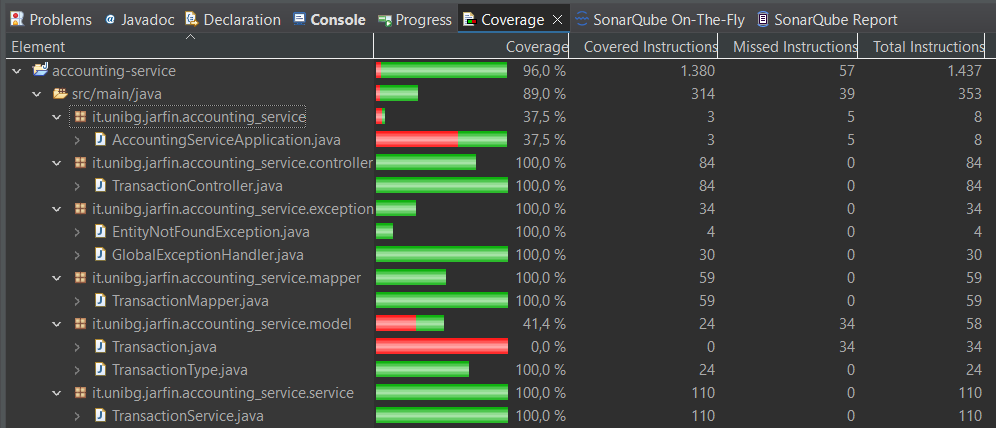
\includegraphics[width=0.9\textwidth]{../Iterazione_1/images/Ecl-accounting-service.png}
    \caption{Report di copertura EclEmma per il microservizio accounting-service}
    \label{fig:eclemma_coverage}
\end{figure}

\subsection{Analisi Architetturale (CodeMR)}

Per valutare la qualità strutturale del microservizio, è stato utilizzato \textbf{CodeMR}. L'analisi ha confermato una costruzione ottima delle classi, evidenziando un basso accoppiamento e un'alta coesione.

\begin{figure}[H]
    \centering
    
\includegraphics[width=0.8\textwidth]{../Iterazione_1/images/quality-attributes.png}
    \caption{Metriche degli attributi di qualità rilevate}
    \label{fig:codemr_quality}
\end{figure}

Il grafico delle dipendenze (Figura \ref{fig:codemr_deps}) offre una rappresentazione visiva delle relazioni tra componenti, confermando una corretta stratificazione tra Controller, Service e Repository.

\begin{figure}[H]
    \centering
    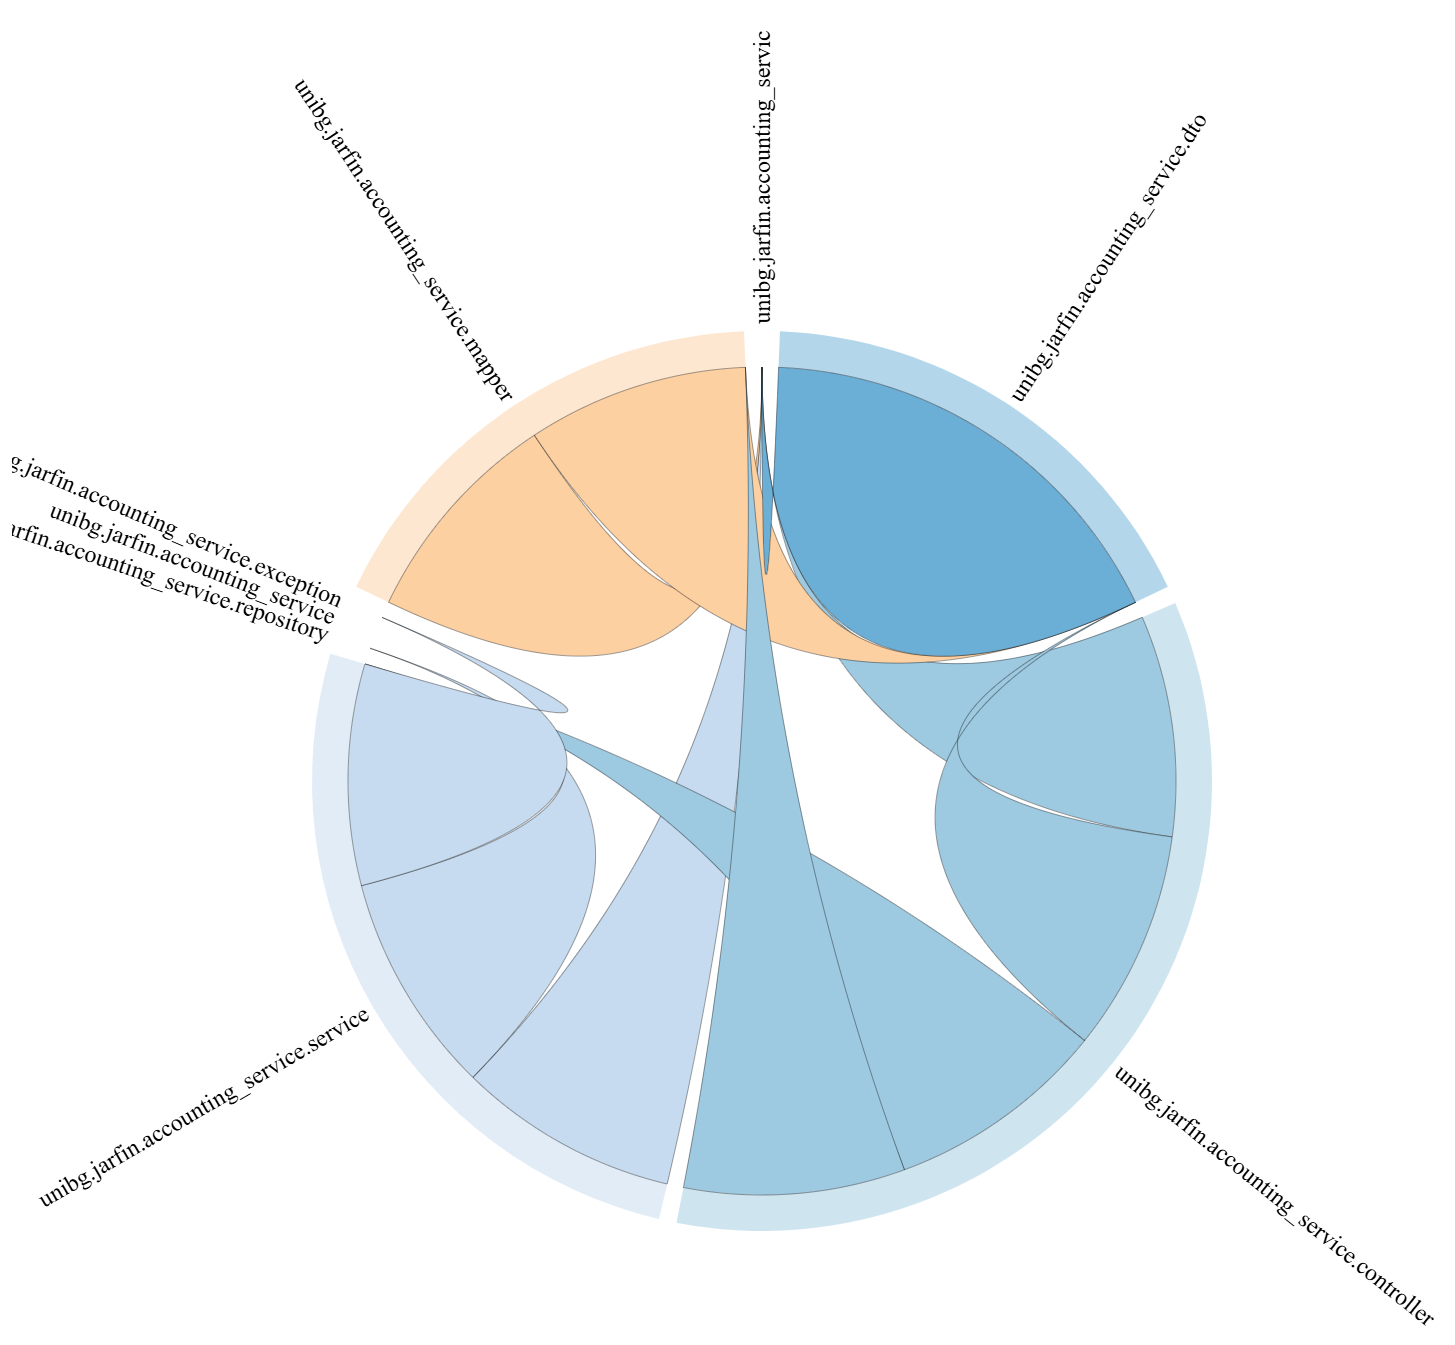
\includegraphics[width=0.9\textwidth]{../Iterazione_1/images/dependencies.png}
    \caption{Grafo delle dipendenze del package Accounting}
    \label{fig:codemr_deps}
\end{figure}

\newpage

\subsection{Integration Testing (Postman)}

A completamento della fase di test, è stata eseguita una validazione \textit{End-to-End} dell'intero stack (Controller + Service + DB + Docker) mediante chiamate REST manuali con \textbf{Postman}.

\textbf{1. Creazione Risorsa (Happy Path)}
Una richiesta \texttt{POST} valida (Figura \ref{fig:post_ok}) restituisce status \texttt{201 Created} e il JSON della transazione salvata, confermando il corretto funzionamento della catena di persistenza.
\begin{figure}[H]
    \centering
    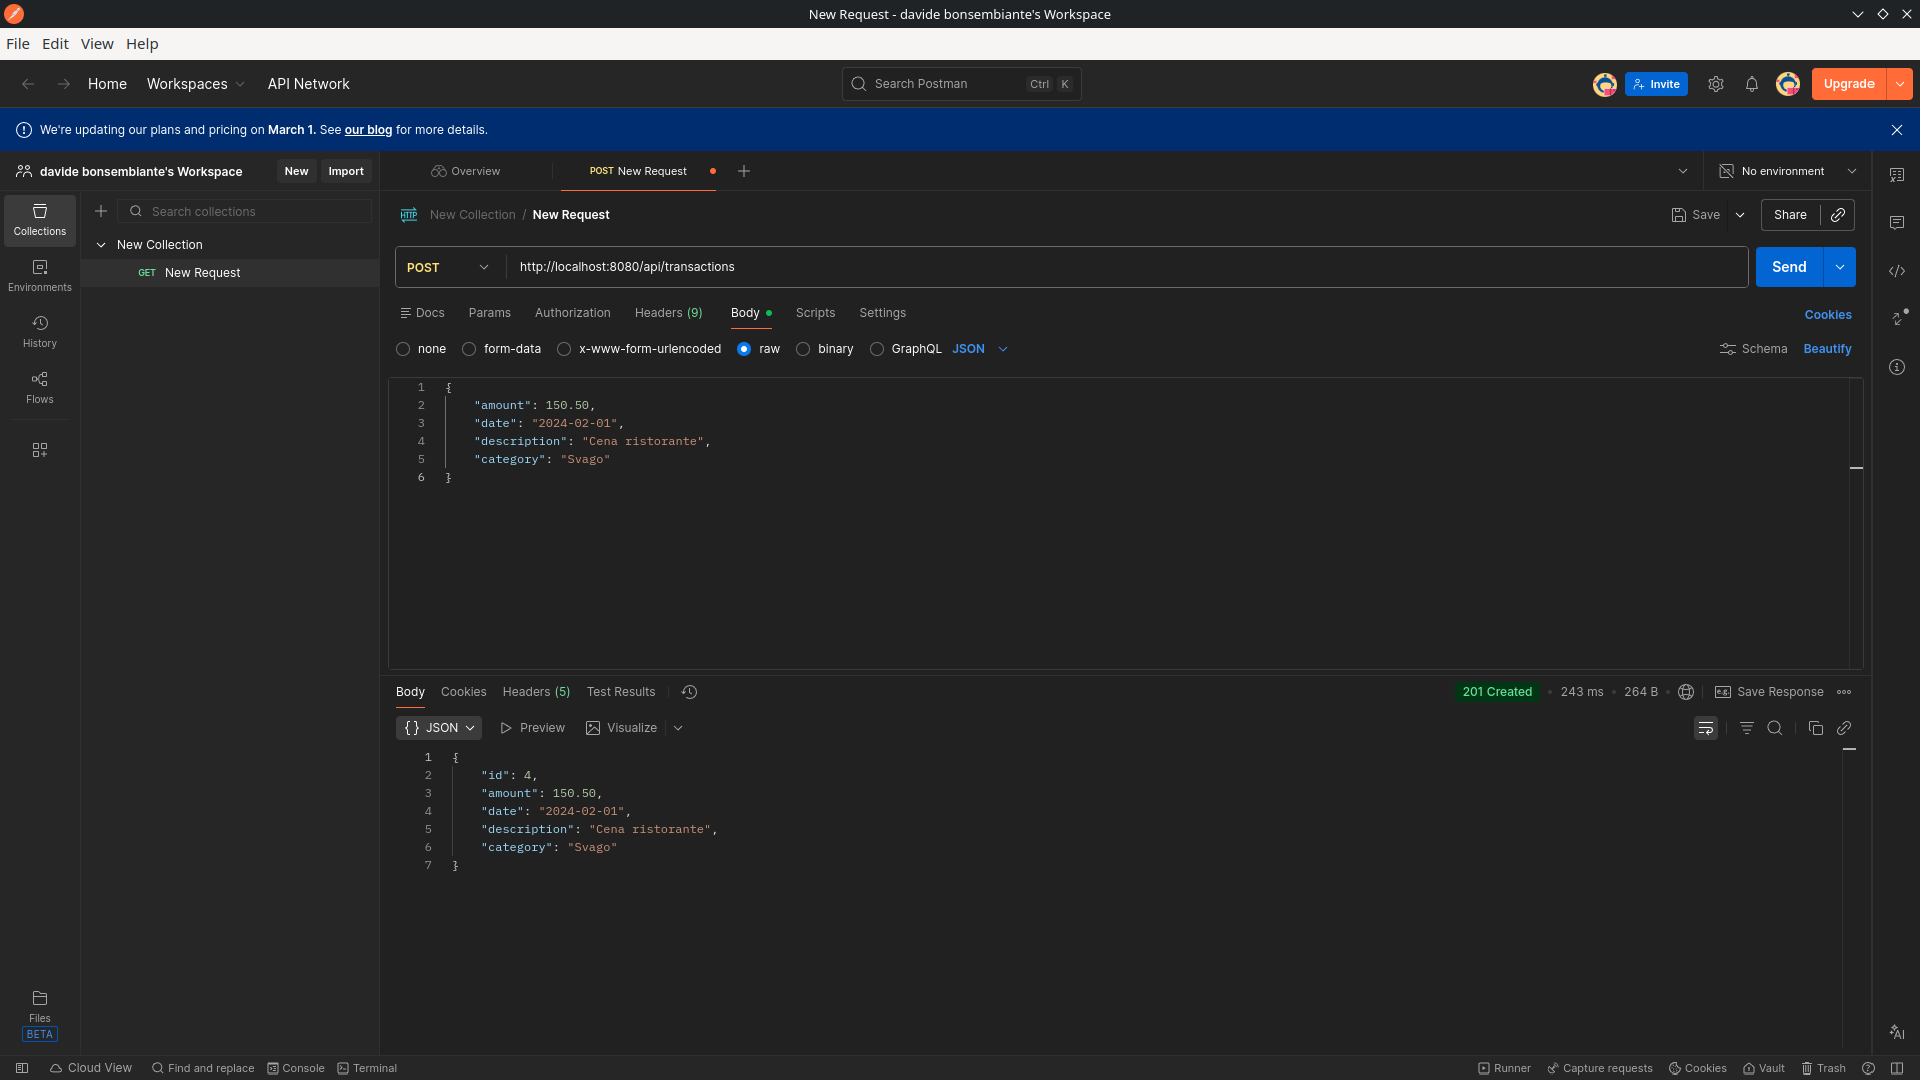
\includegraphics[width=0.85\textwidth]{../Iterazione_1/images/postman_post.png}
    \caption{Creazione di una transazione con successo (Status 201).}
    \label{fig:post_ok}
\end{figure}

\textbf{2. Recupero Dati}
La richiesta \texttt{GET} (Figura \ref{fig:get_ok}) conferma che i dati sono stati persistiti correttamente sul database PostgreSQL containerizzato.
\begin{figure}[H]
    \centering
    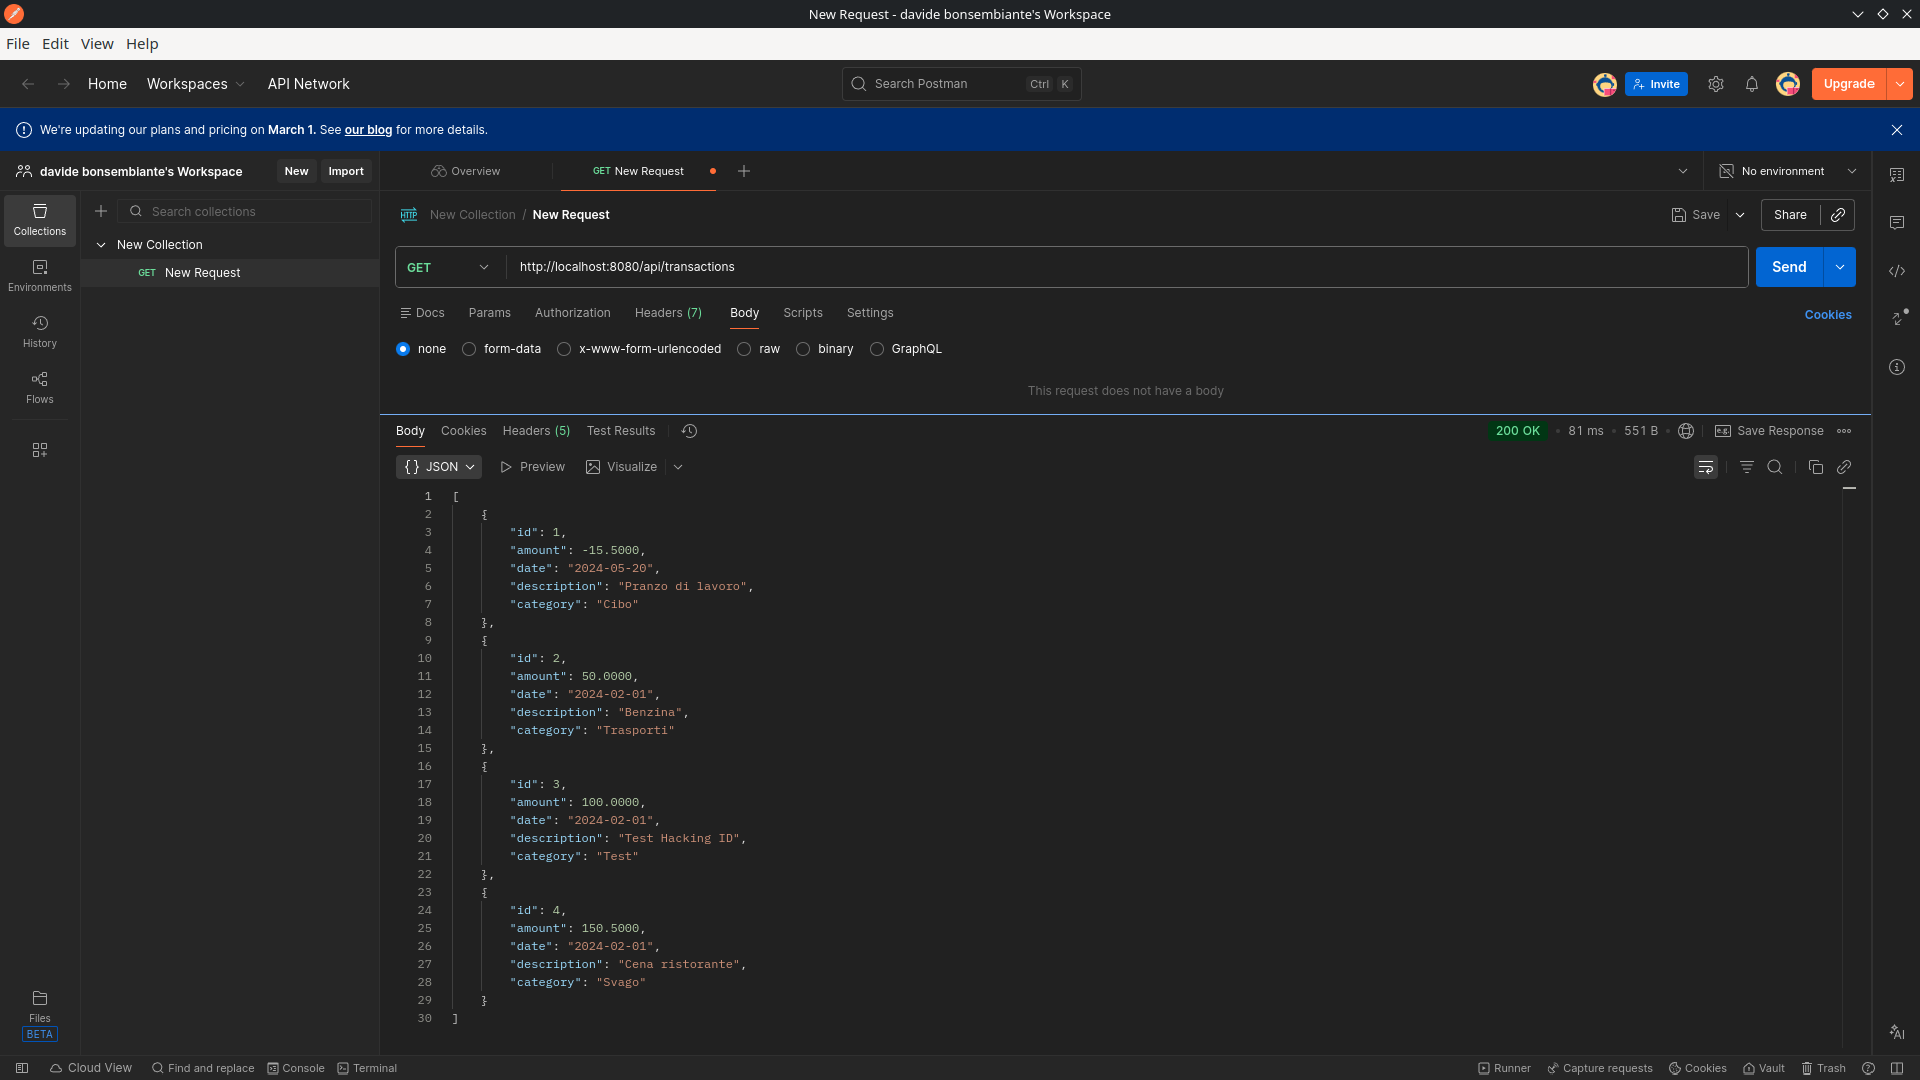
\includegraphics[width=0.85\textwidth]{../Iterazione_1/images/postman_get.png}
    \caption{Recupero della lista delle transazioni (Status 200).}
    \label{fig:get_ok}
\end{figure}

\textbf{3. Validazione Input (Error Handling)}
Inviando un payload con dati non validi (es. importo negativo), il sistema attiva il \texttt{GlobalExceptionHandler} (Figura \ref{fig:post_bad}), restituendo un \texttt{400 Bad Request} con i dettagli dell'errore.
\begin{figure}[H]
    \centering
    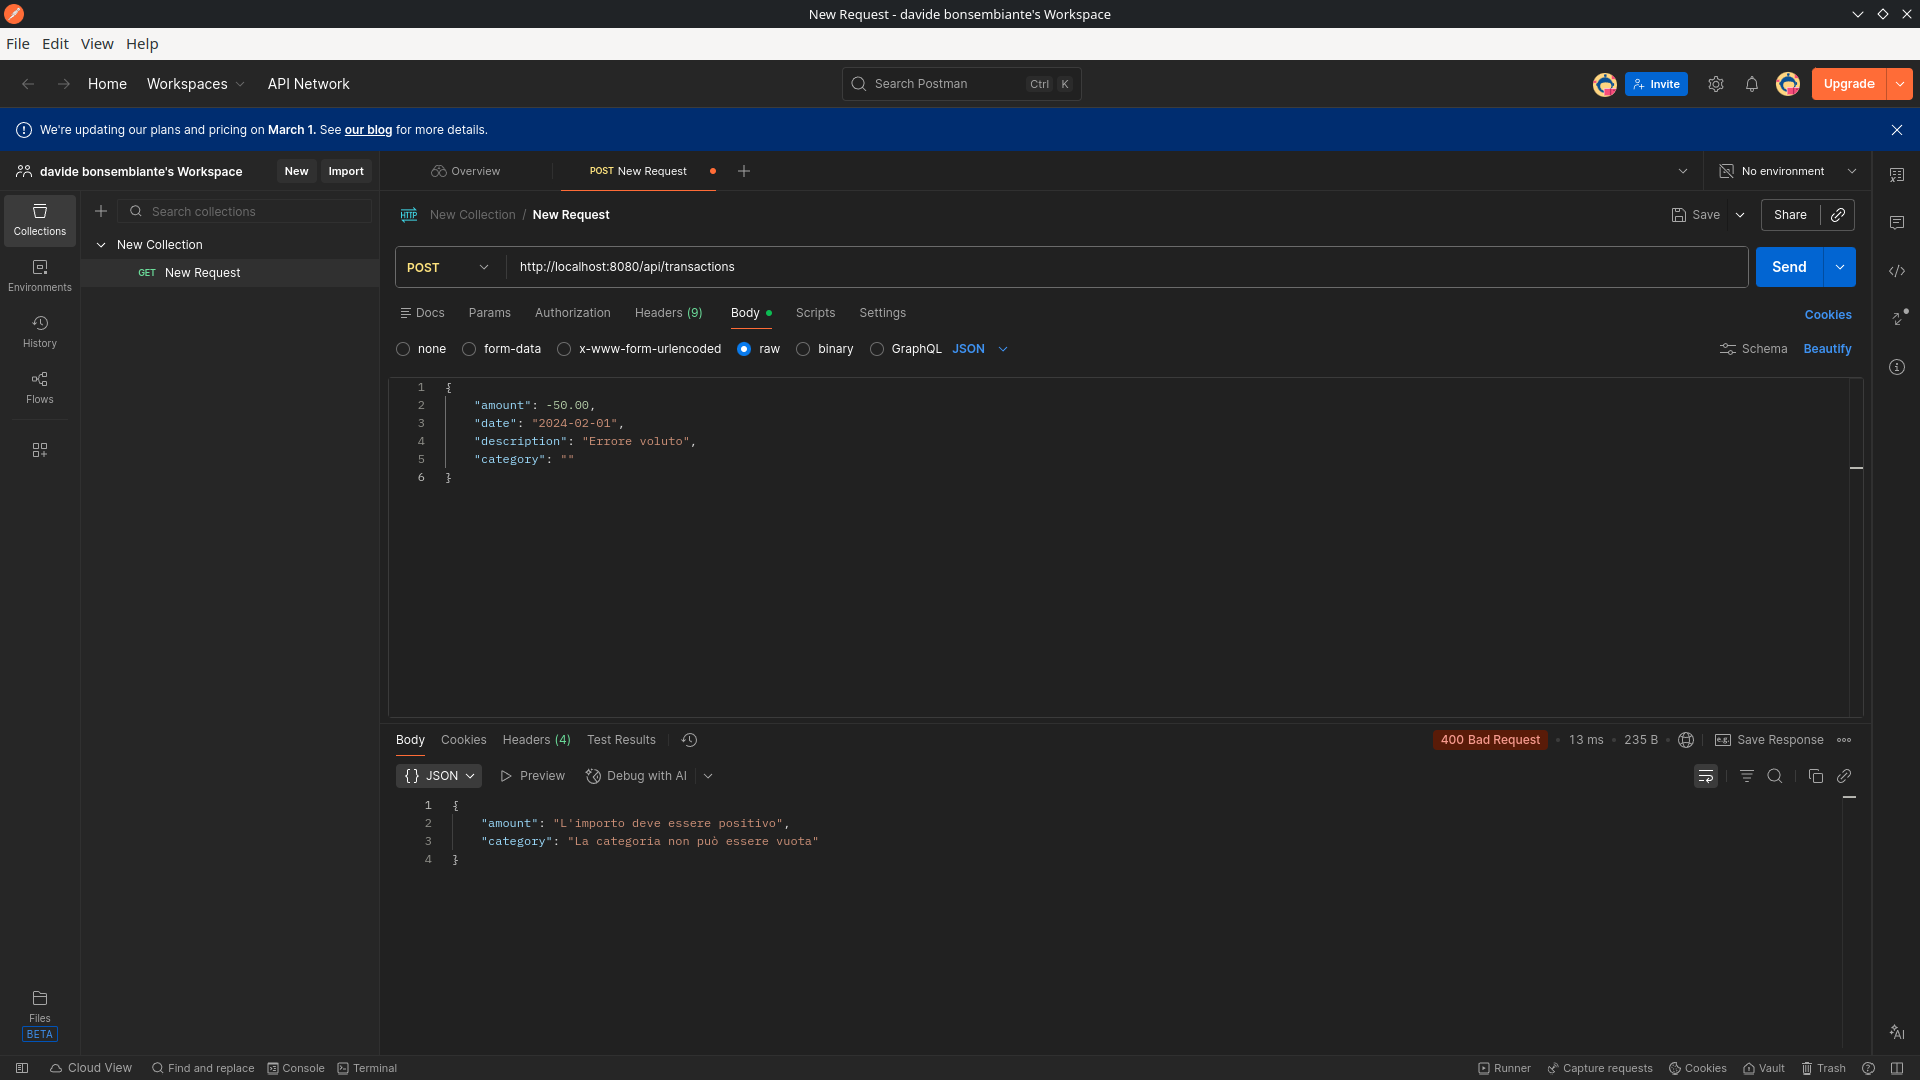
\includegraphics[width=0.85\textwidth]{../Iterazione_1/images/postman_bad_request.png}
    \caption{Test di validazione: risposta 400 Bad Request su importo negativo.}
    \label{fig:post_bad}
\end{figure}

\section{Conclusione Iterazione 1}

L'Iterazione 1 ha consegnato un microservizio di Accounting pienamente operativo, validato sia staticamente che dinamicamente.
L'integrazione di strumenti come SonarLint e CodeMR ha garantito la qualità del codice fin dalle prime fasi, mentre l'alta copertura dei test unitari (96\%) assicura la robustezza della logica di business. Il sistema, containerizzato con Docker e validato via Postman, è ora una base solida pronta per l'integrazione con i moduli di Analytics e Natural Language Understanding.